\documentclass[../main.tex]{subfiles}

\begin{document}

\textbf{Comparison of inference performance}

\begin{figure}[h!]
	\centering
	\subfloat[RMSE of price($x_1$) state \label{fig:4__1__1__RBPF_comparison_rmse_price}]{
		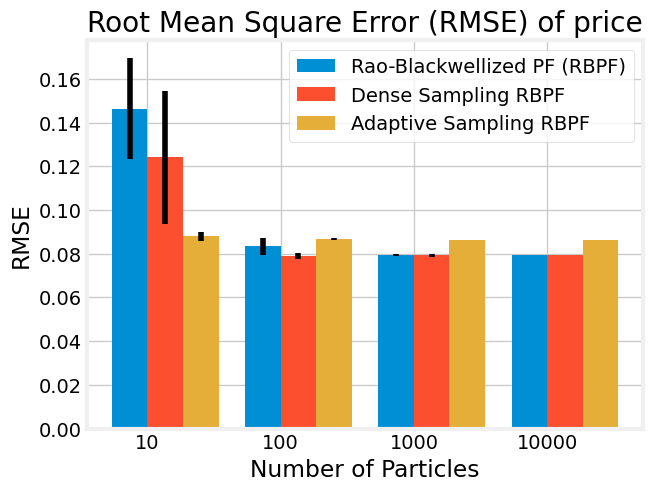
\includegraphics[height=4.5cm]{../plots/4__1__1__RBPF_comparison_rmse_price.png}}
	\qquad
	\subfloat[RMSE of returns($x_2$)  state \label{fig:4__1__1__RBPF_comparison_rmse_returns}]{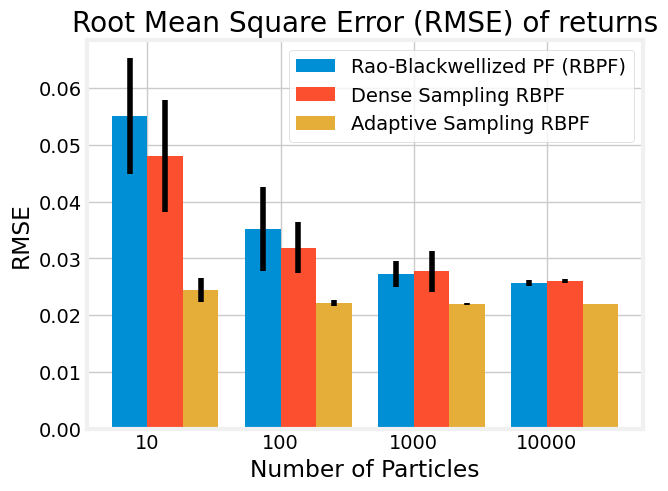
\includegraphics[height=4.5cm]{../plots/4__1__1__RBPF_comparison_rmse_returns.png}}
	
	\qquad
	\subfloat[BPE of returns($x_2$)  state \label{fig:4__1__1__RBPF_comparison_bpe_returns}]{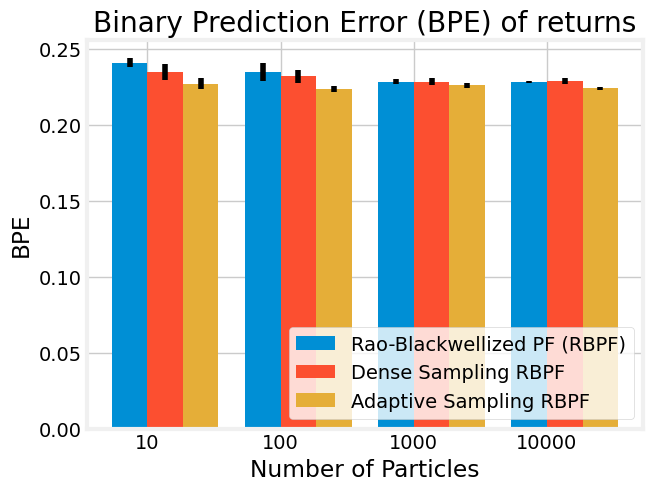
\includegraphics[height=4.5cm]{../plots/4__1__1__RBPF_comparison_bpe_returns.png}}
	\caption{Comparison of inference performance between the 3 RBPF-based particle filters as $N$ varies}
	\label{fig:4__1__1__RBPF_comparison}
\end{figure}

Figure \ref{fig:4__1__1__RBPF_comparison} shows how the performance of the 2 bootstrap particles filters vary as the number of particles, $N$ is changed. 

Firstly, we note that the performance of the 3 RBPF-based particle filters is in general better than the bootstrap particle filters across all performance metrics. This suggests that the ability of the RBPF-based particle filters to marginalise out the gaussian components of the hidden state is very useful in improving the inference performance of the particle filter. 

Secondly, we note that in general, the performance of the dense sampling RBPF and the adaptive sampling RBPF is slightly better than that of the generic RBPF, suggesting that the dense sampling and adaptive sampling improvements are both useful in improving the inference performance of the generic RBPF. Figures \ref{fig:4__1__1__RBPF_comparison_rmse_price} and \ref{fig:4__1__1__RBPF_comparison_rmse_returns} indicate that the performance of the generic RBPF degrades significantly as the number of particles ($N$) used drops, likely due to sample impoverishment. However, the dense sampling RBPF and adaptive sampling RBPF are both more resistant to this degradation in performance, indicating that they are likely less affected by sample impoverishment. 

In particular, the adaptive sampling RBPF is extremely resistant to the degradation in performance as the number of particles drops, with good inference performance even with as low as 10 particles. 

\textbf{Dense Sampling RBPF}

We now examine the reduction in sample impoverishment due to the dense sampling improvement described in \autoref{sec:inference_RBPF}. 

Similarly to \autoref{sec:inference_RBPF}, we demonstrate the problem of sample impoverishment by simulating a single time step of the particle filter, for varying values of $\vt$. Fixing $\mu_k^{(i)}$, $\Sigma_k^{(i)}$ whilst varying $y_k$ and $N$, we simulate one time step of the RBPF update step described above and present the normalised entropy of the RBPF particle weights with and without the dense sampling improvement in Figure \ref{fig:2__2__2__sample_impoverishment}.

\begin{figure}[h!]
	\centering
	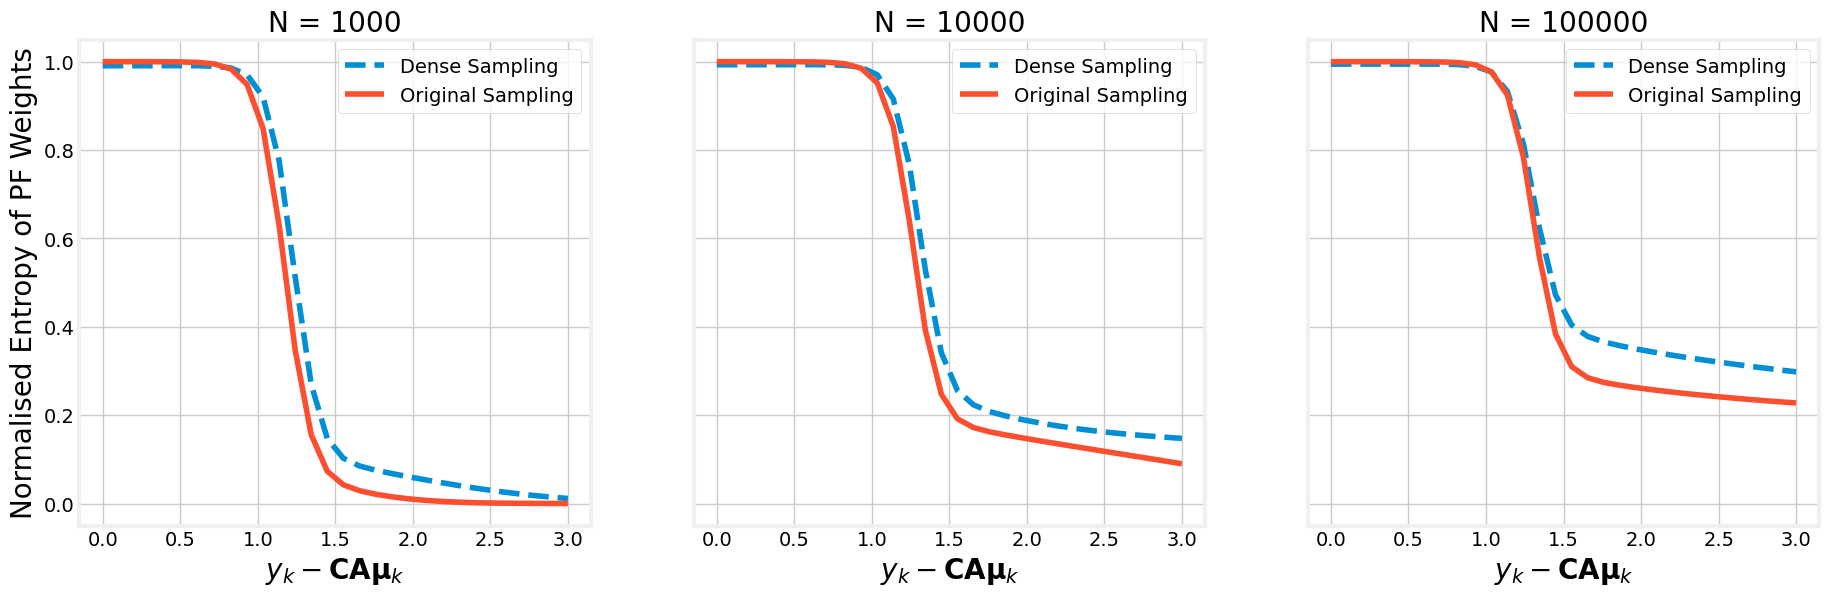
\includegraphics[width=15.0cm]{../plots/4__1__1__dense_sampling.png}
	\caption{Improvement in normalised entropy of RBPF particle weights using dense sampling with hyperparameters: ($\epsilon_\lambda = 0.1$, $m=2$)}
	\label{fig:4__1__1__dense_sampling}
\end{figure}	

We can see from Figure \ref{fig:2__2__2__sample_impoverishment} that the dense sampling improvement causes the normalised entropy of the RBPF particle weights to increase for larger price outliers $\vt$. A higher normalised entropy indicates that the weights of the RBPF particles are more evenly distributed and hence that there are a larger number of particles with effective weights under the dense sampling improvement.
	
\textbf{Adaptive Sampling RBPF}

\begin{figure}[h!]
	\centering
	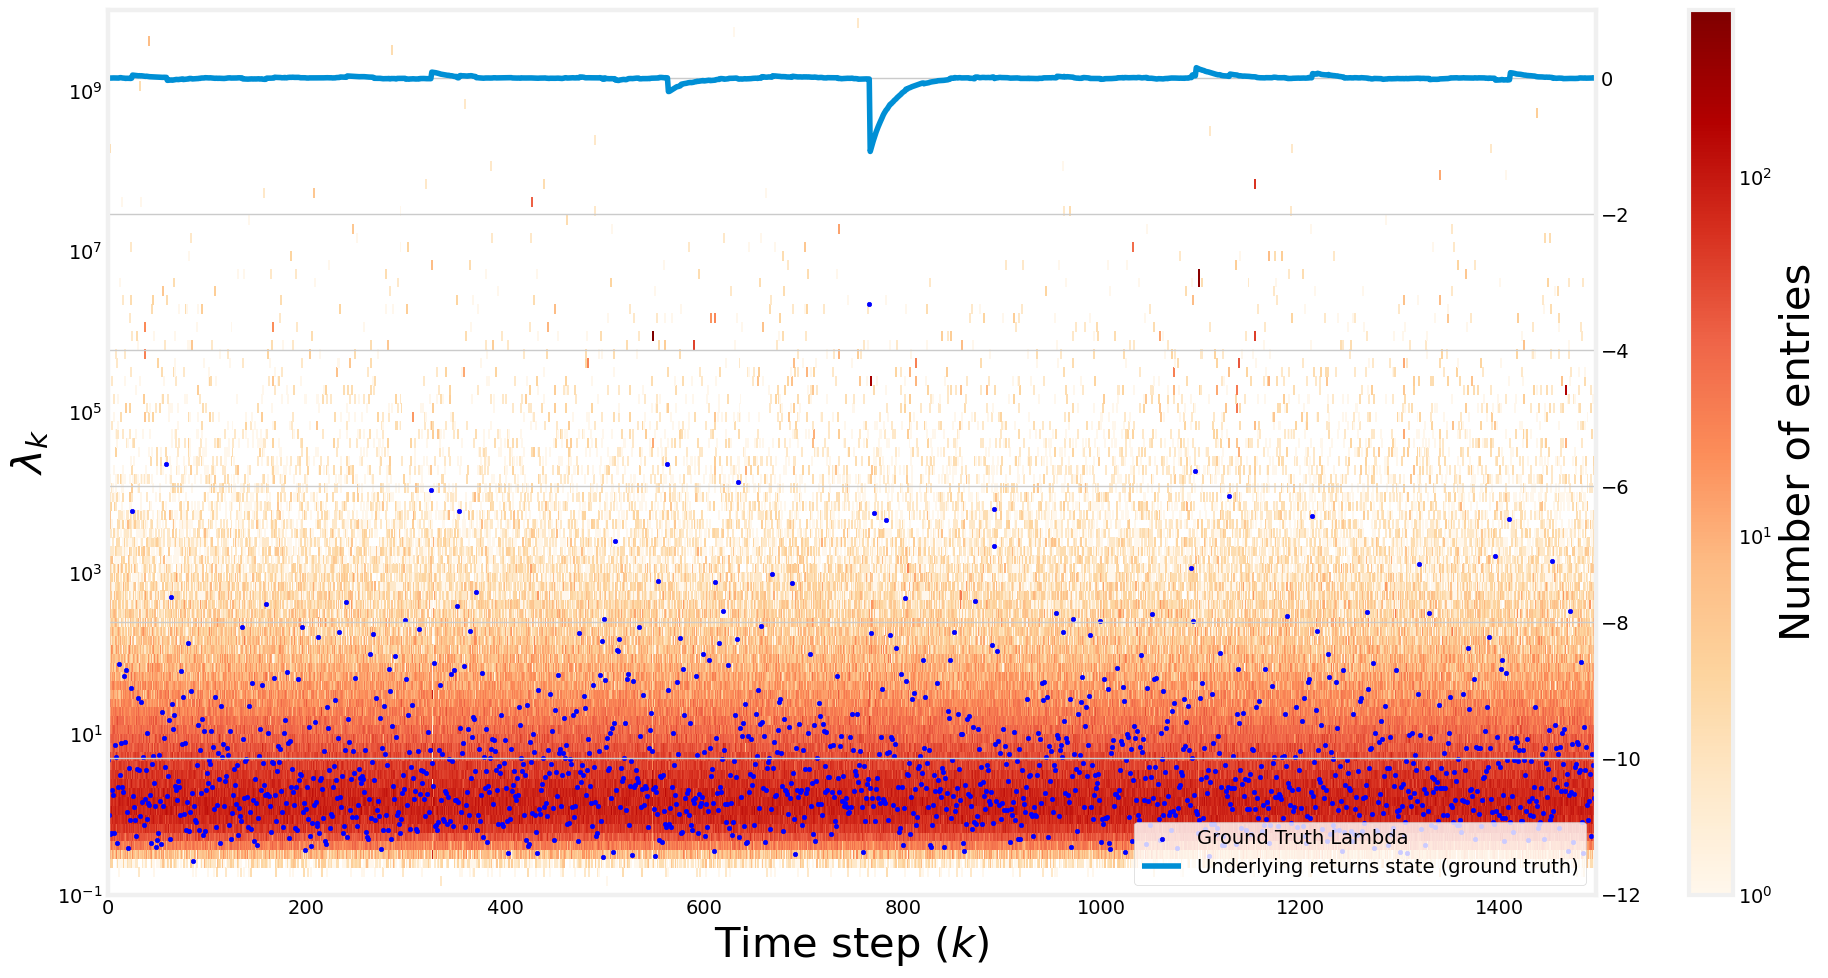
\includegraphics[width=15.0cm]{../plots/4__1__1__lambdas_generic.png}
	\caption{Distribution of samples $\lambda_k^{(i)}$ from the Generic RBPF}
	\label{fig:4__1__1__lambdas_generic}
\end{figure}

\begin{figure}[h!]
	\centering
	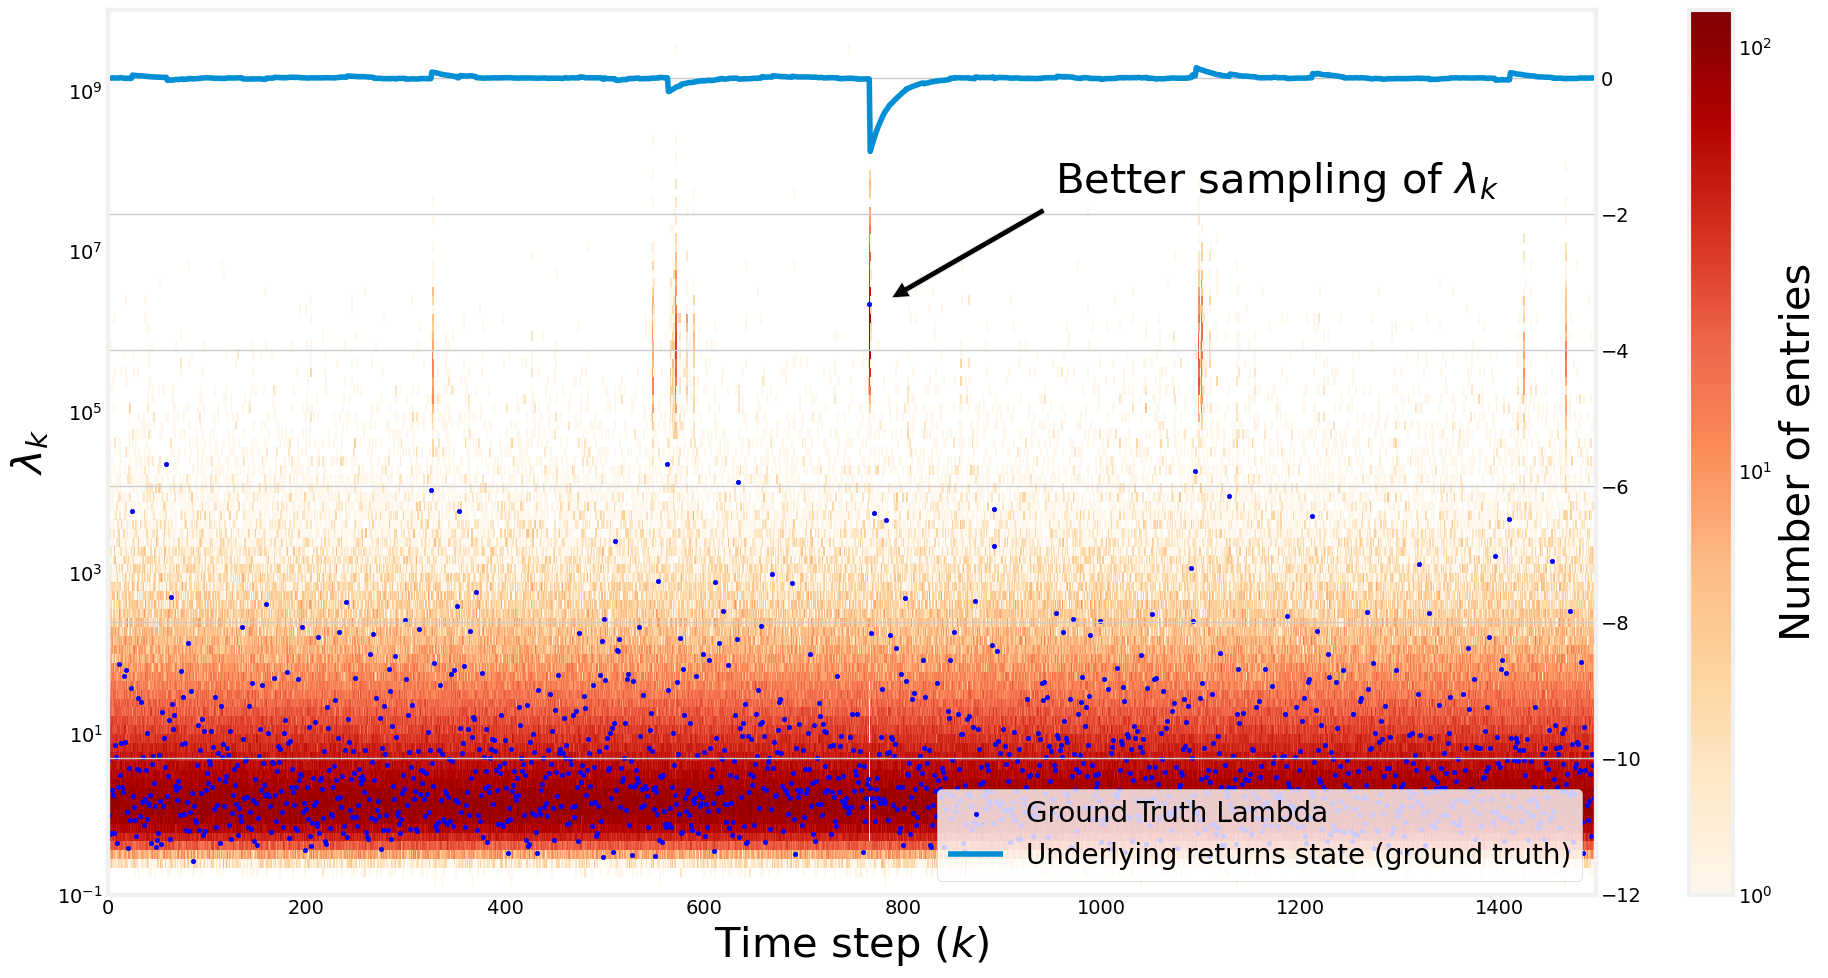
\includegraphics[width=15.0cm]{../plots/4__1__1__lambdas_adaptive_sampling.png}
	\caption{Distribution of samples $\lambda_k^{(i)}$ from the Adaptive Sampling RBPF}
	\label{fig:4__1__1__lambdas_adaptive_sampling}
\end{figure}

Figure \ref{fig:4__1__1__lambdas_generic} shows the distribution of samples $\lambda_k^{(i)}$ from the Adaptive Sampling RBPF as well as the ground truth $\lambda_k$ used to generate the simulation data. 
Figure \ref{fig:4__1__1__lambdas_adaptive_sampling} shows a similar figure for the generic RBPF $\textit{after}$ the resampling step. 

Comparing Figures \ref{fig:4__1__1__lambdas_generic} and \ref{fig:4__1__1__lambdas_adaptive_sampling}, we can see qualitatively that the distribution of samples from the Adaptive Sampling RBPF is distributed more closely around the ground truth $\lambda_k$, resulting in a many more effective samples being generated using the Adaptive Sampling RBPF compared to the generic RBPF.

Note the extremely challenging nature of forming a good importance sampling estimate of the posterior $p(\lambda_k | y_k, \mu_{k-1}, \Sigma_{k-1})$ using only samples from the prior as $\lambda_k$ ranges over 7 orders of magnitude ($10^{-1}$ to $10^7$) in this example. This makes it very difficult to form a good discrete importance sampling estimate, which would require a huge amount of particles to cover the entire possible range of $\lambda_k$ (which theoretically has infinite support). With the adaptive sampling improvement, we are able to use the information from the current observation to sample directly from the approximate posterior, which increases the sampling efficiency of the particle filter greatly. 

We next investigate how few particles we can use with the new adaptive sampling particle filter before performance degrades unacceptably. Figure \ref{fig:4__1__1__very_small_N} shows how the RMSE of the inferred underlying returns process changes for very low values of $N$. Interestingly, we note that the adaptive sampling RBPF is still capable of good inference performance even with extremely low $N = 4$, unlike the generic RBPF, which suffers from degradation of inference performance when using a low number of particles. 

\begin{figure}[h!]
	\centering
	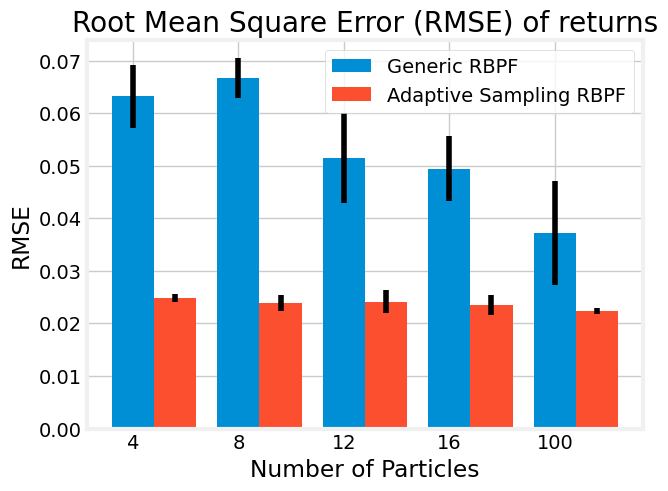
\includegraphics[width=12.0cm]{../plots/4__1__1__very_small_N.png}
	\caption{Performance of the RBPF-based particle filters for very low $N$}
	\label{fig:4__1__1__very_small_N}
\end{figure}
	
\end{document}